\documentclass[11pt]{article} % use larger type; default would be 10pt

\usepackage[utf8]{inputenc} % set input encoding (not needed with XeLaTeX)
\usepackage{graphicx}


\begin{document}

\section{Quadcopter Mechanics}

The defining feature of a quadcopter is that it has four spinning blades which provide thrust. This has certain advantages and disadvantages. One advantage is that a quadcopter provides a very stable airframe. A fixed wing aircraft must maintain a certain velocity to stay airborn, whereas a quadcopter can essentially hover in place. The ability to move more slowly than a fixed wing aircraft makes a quadcopter a good choice for navigating an environment in which it is unsure of its path. Rather than being forced to make quick decisions at a high velocity, a quadcopter has the luxury of taking its time, stopping to make sure it is not about to collide with an obstacle. The number of blades used is somewhat arbitrary, but quadcopters are a good compromise between cost and reliability. A copter with three rotors might not be powerful or versatile enough, whereas a quadcopter is powerful enough to carry a payload without being too expensive or heavy to realistically construct.

A quadcopter moves and rotates on all three axes, as seen in Fig. 1.

\begin{figure}[h!]
	\centering
  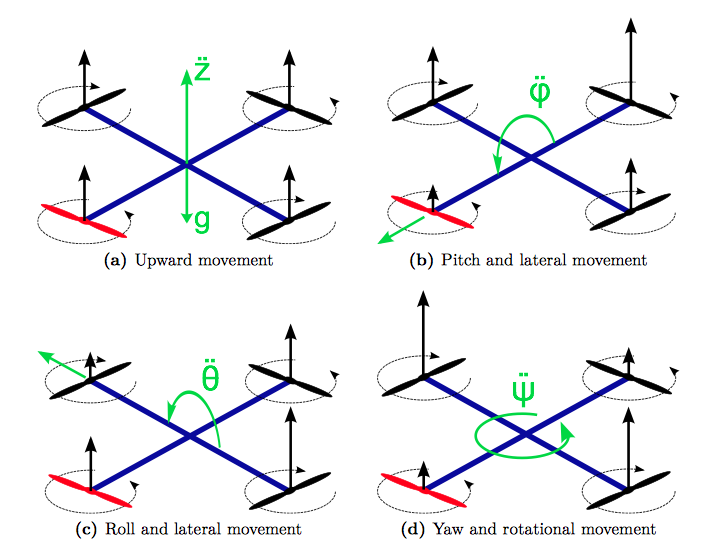
\includegraphics[width=345px]{quadcopter_movement.png}
  \caption{Quadcopter movement}
  \label{fig:}
\end{figure} 

Movement up or down is controlled by increasing or decreasing the thrust of all props equally. Sideways movement is acheived by increasing the movement of one prop and decreasing the opposite prop, pitching the quadcopter in the direction of the reduced lift. The changed angle of the props results in a horizontal component to the thrust. Yaw is more complicated; A quadcopter is designed so that each pair of opposite rotors spins in the same direction, two clockwise and two counterclockwise. When a pair of rotors spin, they increase the angular momentum of the entire quadcopter system in a certain direction. This effect is normally cancelled out by the fact that 2 props are spinning in the opposite direction of the other two, but increasing the power to two spinning in the same direction while decreasing the other two increasing the angular momentum of all of the propellers in a certain direction. Because angular momentum is always conserved, this means that the rest of the quadcopter has to rotate in the opposite direction to cancel out the increased momentum of the propellers, resulting in a yaw, or rotation of the entire aircraft. Barrel rolls can be accomplished by extreme amounts of pitch (DO NOT ATTEMPT).

\end{document}
